\documentclass [PhD] {uclathes}

% \newcommand{\hvecf}{{\mathbf h}}
\newcommand{\bvecf}{{\mathbf b}}
\newcommand{\pvecf}{{\mathbf p}}
\newcommand{\kvecf}{{\mathbf k}}
\newcommand{\wvecf}{{\mathbf w}}
\newcommand{\nvecf}{{\mathbf n}}
\newcommand{\qvecf}{{\mathbf q}}
\newcommand{\yvecf}{{\mathbf y}}
\newcommand{\cvecf}{{\mathbf c}}
\newcommand{\zvecf}{{\mathbf z}}
\newcommand{\uvecf}{{\mathbf u}}
\newcommand{\vvecf}{{\mathbf v}}
\newcommand{\mvecf}{{\mathbf m}}
\newcommand{\avecf}{{\mathbf a}}
\newcommand{\lvecf}{{\mathbf l}}
\newcommand{\xvecf}{{\mathbf x}}
\newcommand{\Gvecf}{{\mathbf G}}
\newcommand{\dvecf}{{\mathbf d}}
\newcommand{\evecf}{{\mathbf e}}
\newcommand{\tvecf}{{\mathbf t}}
\newcommand{\svecf}{{\mathbf s}}
\newcommand{\rvecf}{{\mathbf r}}
\newcommand{\gvecf}{{\mathbf g}}
%\newcommand{\hvec}{{\mathrm h}}
%\newcommand{\bvec}{{\mathrm b}}
%\newcommand{\pvec}{{\mathrm p}}
%\newcommand{\kvec}{{\mathrm k}}
%\newcommand{\wvec}{{\mathrm w}}
%\newcommand{\nvec}{{\mathrm n}}
%\newcommand{\qvec}{{\mathrm q}}
%\newcommand{\yvec}{{\mathrm y}}
%\newcommand{\cvec}{{\mathrm c}}
%\newcommand{\zvec}{{\mathrm z}}
%\newcommand{\uvec}{{\mathrm u}}
%\newcommand{\vvec}{{\mathrm v}}
%\newcommand{\mvec}{{\mathrm m}}
%\newcommand{\avec}{{\mathrm a}}
%\newcommand{\lvec}{{\mathrm l}}
%\newcommand{\xvec}{{\mathrm x}}
%\newcommand{\dvec}{{\mathrm d}}
%\newcommand{\evec}{{\mathrm e}}
%\newcommand{\tvec}{{\mathrm t}}
%\newcommand{\svec}{{\mathrm s}}
%\newcommand{\rvec}{{\mathrm r}}
%\newcommand{\gvec}{{\mathrm g}}

\newcommand{\hvec}{{h}}
\newcommand{\bvec}{{b}}
\newcommand{\pvec}{{p}}
\newcommand{\kvec}{{k}}
\newcommand{\wvec}{{w}}
\newcommand{\nvec}{{n}}
\newcommand{\qvec}{{q}}
\newcommand{\yvec}{{y}}
\newcommand{\cvec}{{c}}
\newcommand{\zvec}{{z}}
\newcommand{\uvec}{{u}}
\newcommand{\vvec}{{v}}
\newcommand{\mvec}{{m}}
\newcommand{\avec}{{a}}
\newcommand{\lvec}{{l}}
\newcommand{\xvec}{{x}}
\newcommand{\dvec}{{d}}
\newcommand{\evec}{{e}}
\newcommand{\tvec}{{t}}
\newcommand{\svec}{{s}}
\newcommand{\rvec}{{r}}
\newcommand{\gvec}{{g}}
\newcommand{\Gvec}{{\mathrm G}}
\newcommand{\lambdavec}{$$\mbox{\boldmath$\lambda$}$$}
\newcommand{\Thetamat}{{\mathbf \Theta}}
\newcommand{\Phimat}{{\mathbf \Phi}}
\newcommand{\Deltamat}{{\mathbf \Delta}}
\newcommand{\Sigmamat}{{\mathbf \Sigma}}
\newcommand{\Omegamat}{{\mathbf \Omega}}
\newcommand{\Psimat}{{ \Psi}}
\newcommand{\Pimat}{{\mathbf \Pi}}
\newcommand{\Gammamat}{{\mathbf \Gamma }}
\newcommand{\Lambdamat}{{\mathbf \Lambda}}
\newcommand{\epsilonvec}{{\mathbf \epsilon}}
\newcommand{\etavec }{{\mathbf \eta }}
\newcommand{\zeromat }{{\mathbf 0 }}
\newcommand{\Zeromat }{{\mathbf 0 }}
%\newcommand{\log10}{{\log_{10}}}
\newcommand{\Gmat}{{G}}
\newcommand{\Omat}{{O}}
\newcommand{\Mmat}{{M}}
\newcommand{\Lmat}{{L}}
\newcommand{\Emat}{{E}}
\newcommand{\Vmat}{{V}}
\newcommand{\Kmat }{{K}}
\newcommand{\Fmat }{{F}}
\newcommand{\Bmat}{{B}}
\newcommand{\Cmat}{{C}}
\newcommand{\Hmat}{{H}}
\newcommand{\Imat}{{\mathbf I}}
\newcommand{\Dmat}{{D}}
\newcommand{\Qmat}{{Q}}
\newcommand{\Rmat}{{R}}
\newcommand{\Jmat}{{J}}
\newcommand{\Xmat}{{X}}
\newcommand{\Nmat}{{N}}
\newcommand{\Amat}{{A}}
\newcommand{\Ymat}{{Y}}
\newcommand{\Wmat}{{W}}
\newcommand{\Umat}{{U}}
\newcommand{\Tmat}{{T}}
\newcommand{\Smat}{{S}}
\newcommand{\Zmat}{{Z}}
\newcommand{\Pmat}{{P}}
%\newcommand{\Gmat}{{\mathrm G}}
%\newcommand{\Omat}{{\mathrm O}}
%\newcommand{\Mmat}{{\mathrm M}}
%\newcommand{\Lmat}{{\mathrm L}}
%\newcommand{\Emat}{{\mathrm E}}
%\newcommand{\Vmat}{{\mathrm V}}
%\newcommand{\Kmat }{{\mathrm K}}
%\newcommand{\Fmat }{{\mathrm F}}
%\newcommand{\Bmat}{{\mathrm B}}
%\newcommand{\Cmat}{{\mathrm C}}
%\newcommand{\Hmat}{{\mathrm H}}
%\newcommand{\Imat}{{\mathrm I}}
%\newcommand{\Dmat}{{\mathrm D}}
%\newcommand{\Qmat}{{\mathrm Q}}
%\newcommand{\Rmat}{{\mathrm R}}
%\newcommand{\Jmat}{{\mathrm J}}
%\newcommand{\Xmat}{{\mathrm X}}
%\newcommand{\Nmat}{{\mathrm N}}
%\newcommand{\Amat}{{\mathrm A}}
%\newcommand{\Ymat}{{\mathrm Y}}
%\newcommand{\Wmat}{{\mathrm W}}
%\newcommand{\Umat}{{\mathrm U}}
%\newcommand{\Tmat}{{\mathrm T}}
%\newcommand{\Smat}{{\mathrm S}}
%\newcommand{\Zmat}{{\mathrm Z}}
%\newcommand{\Pmat}{{\mathrm P}}
\newcommand{\Gmatf}{{\mathbf G}}
\newcommand{\Omatf}{{\mathbf O}}
\newcommand{\Mmatf}{{\mathbf M}}
\newcommand{\Lmatf}{{\mathbf L}}
\newcommand{\Ematf}{{\mathbf E}}
\newcommand{\Vmatf}{{\mathbf V}}
\newcommand{\Rmatf}{{\mathbf R}}
\newcommand{\Kmatf }{{\mathbf K}}
\newcommand{\Fmatf }{{\mathbf F}}
\newcommand{\Hmatf}{{\mathbf H}}
\newcommand{\Imatf}{{\mathbf I}}
\newcommand{\Dmatf}{{\mathbf D}}
\newcommand{\Qmatf}{{\mathbf Q}}
\newcommand{\Jmatf}{{\mathbf J}}
\newcommand{\Xmatf}{{\mathbf X}}
\newcommand{\Nmatf}{{\mathbf N}}
\newcommand{\Amatf}{{\mathbf A}}
\newcommand{\Ymatf}{{\mathbf Y}}
\newcommand{\Wmatf}{{\mathbf W}}
\newcommand{\Umatf}{{\mathbf U}}
\newcommand{\Tmatf}{{\mathbf T}}
\newcommand{\Smatf}{{\mathbf S}}
\newcommand{\Zmatf}{{\mathbf Z}}
\newcommand{\Pmatf}{{\mathbf P}}
\newcommand{\Bmatf}{{\mathbf B}}
\newcommand{\Cmatf}{{\mathbf C}}
\newcommand{\be }{\begin{equation}}
\newcommand{\ee }{\end{equation}}
\newcommand{\beqn }{\begin{eqnarray}}
\newcommand{\eeqn }{\end{eqnarray}}
                         % personal LaTeX macros
\usepackage{graphicx}

%%%%%%%%%%%%%%%%%%%%%%%%%%%%%%%%%%%%%%%%%%%%%%%%%%%%%%%%%%%%%%%%%%%%%%
%
% Usually things live in separate flies.
%
% \input {prelim}                           % preliminary page info

%%%%%%%%%%%%%%%%%%%%%%%%%%%%%%%%%%%%%%%%%%%%%%%%%%%%%%%%%%%%%%%%%%%%%%%%
%                                                                      %
%                          PRELIMINARY PAGES                           %
%                                                                      %
%%%%%%%%%%%%%%%%%%%%%%%%%%%%%%%%%%%%%%%%%%%%%%%%%%%%%%%%%%%%%%%%%%%%%%%%

\title          {High-Speed Imaging and Optical Sensing Systems for Biomedical Applications}
\author         {Ata Mahjoubfar}
% Note: department is really your area of research.  I.e. leave out 'Department of'.
\department     {Electrical Engineering}
% Note:  degreeyear should be optional, but as of  5-Feb-96
% it seems required or you get a year of ``2''.   -johnh
\degreeyear     {2014}

%%%%%%%%%%%%%%%%%%%%%%%%%%%%%%%%%%%%%%%%%%%%%%%%%%%%%%%%%%%%%%%%%%%%%%%%

\chair          {Bahram Jalali}
\member         {Benjamin S. Williams}
\member         {Katsushi Arisaka}
\member         {Kayvan Niazi}
\member         {Tatsuo Itoh}
\member         {Dean Ho}

%%%%%%%%%%%%%%%%%%%%%%%%%%%%%%%%%%%%%%%%%%%%%%%%%%%%%%%%%%%%%%%%%%%%%%%%

\dedication     {\textsl{To my parents \ldots \\
                who---among so many other things--- \\
                got a loan to buy me a computer \\
                when I was in high school}}

%%%%%%%%%%%%%%%%%%%%%%%%%%%%%%%%%%%%%%%%%%%%%%%%%%%%%%%%%%%%%%%%%%%%%%%%

\acknowledgments {First and foremost, I would like to express my sincere gratitude to my advisor, Prof. Bahram Jalali, for his immeasurable amount of support and guidance. His patience, vast and deep knowledge of numerous fields, and attention to fundamentals has always inspired me. His training has significantly influenced my character both in professional and personal life. 

Wholeheartedly, I thank Prof. Kayvan Niazi. His knowledge, his passion for teaching, and above all, his spirit has been inspirational. His insightful feedback and guidance, specifically on biological, studies were critical in completing this work. Also, I would like to thank my other committee members, Prof. Tatsuo Itoh, Prof. Katsushi Arisaka, Prof. Benjamin S. Williams, and Prof. Dean Ho, for their invaluable time and feedback.

I would like to thank impressive students and postdocs of Prof. Jalali's research group, who I have learned alot from. Specifically, Keisuke Goda and Daniel Solli had a significant influence on shaping me into a scientist. Also, I am very thankful to Eric Diebold, Kevin K. Tsia, Jost Adam, Ali Fard, Ali Ayazi, Niusha Sarkhosh, Kam Yan Hon, and Alexander Weidel for the helpful discussions that we had. I would like to express my appreciatation for the help of our undergraduate students, especially Allen Huang, Li-Chia Tai, and Jim Lin who have dedicated significant amount of time and effort to my project. Last, but not least, I am truly grateful of my colleague graduate student, Claire Lifan Chen, who has worked with me through good and bad times of many projects. Without her help, I could have never achieved many of my celebrated results.

I would like to thank all of my publication co-authors, which our works consist many chapters of this dissertation. Chapter 1 is a version of Applied Physics Letters, Vol. 98, No. 10, 101107, 2011. Chapter 2 is a version of Proceedings of SPIE, Frontiers in Ultrafast Optics: Biomedical, Scientific, and Industrial Applications XIII, San Francisco, CA, 2013, 86110N, which is a collaborative work between Prof. Bahram Jalali and Prof. Dino di Carlo’s groups. Chapter 3 is a version of Biomedical Optics Express, Vol. 4, No. 9, pp. 1618-1625, 2013. Chapter 4 is a version of Journal of the Optical Society of America A, Vol. 30, No. 10, pp. 2124-2132, 2013. Finally, Chapter 5 is a version of Conference on Lasers and Electro-Optics (CLEO), San Jose, CA, 2010, CFA4.

I also had many great mentors over the course of my undergraduate education who led me to this PhD in Electrical Engineering. In particular, I am very grateful of Prof. Mahmoud Shahabadi, Prof. Mohammad Yavari, and Prof. Zainalabedin Navabi. 

Furthermore, I would like to thank my friends Yunan Zhu and Zohreh Khodaparast whose support gave me the strength, energy, and drive to go through difficulties of this program. Finally, I would like to thank my roommate, Arash Mirhaj for productive technical and non-technical discussions over many late night working hours. 

Most important of all, I am supremely grateful to my family for their unconditional love and support. They have sacrificed so much for me to be here. My mom, Azarjoun, has been my role model for being reliable, hardworking, and hopeful while I learned being thorough from my dad. My sister, Maryam has been a constant source of love, and My brother, Ali has always supported my curiosity... Azarjoun, Baba, Maryam, and Ali! You helped me whenever I needed it. Thank you for always being there.
}

%%%%%%%%%%%%%%%%%%%%%%%%%%%%%%%%%%%%%%%%%%%%%%%%%%%%%%%%%%%%%%%%%%%%%%%%

%
% UCLA Policy on Vita
% For security reasons, UCLA policy specifies that your birth year and birth place should not be included in your vita.
%
\vitaitem   {2005}
                {Intern, Department of Electrical Energy, Systems and Automation, Gent University, Belgium.}
\vitaitem   {2006}
                {B.Sc., Electrical Engineering, University of Tehran, Iran.}
\vitaitem   {2008}
                {M.Sc., Electrical Engineering, University of Tehran, Iran.}
\vitaitem   {2009--2011}
                {Teaching Assistant, Electrical Engineering Department, UCLA.}
\vitaitem   {2013--2014}
                {Teaching Associate, Electrical Engineering Department, UCLA.}
\vitaitem   {2009--present}
                {Graduate Student Researcher, Electrical Engineering Department, UCLA.}
\vitaitem   {2010--present}
                {Graduate Student Researcher, California NanoSystems Institute, Los Angeles.}

%%%%%%%%%%%%%%%%%%%%%%%%%%%%%%%%%%%%%%%%%%%%%%%%%%%%%%%%%%%%%%%%%%%%%%%%


\publication   {J. Chan, \textbf{A. Mahjoubfar}, M. Asghari, and B. Jalali, ``\textit{Reconstruction in time-bandwidth compression systems,}'' Applied Physics Letters, Vol. 105, No. 22, 221105, 2014.}

\presentation   {A. Yazaki, \textbf{A. Mahjoubfar}, C. Kim, J. Chan, K. Goda, M. Watanabe, and B. Jalali, ``\textit{Ultrafast web-inspecting laser scanner,}'' Progress In Electromagnetics Research Symposium, Guangzhou, China, 2014, 140319211016.}

\presentation   {\textbf{A. Mahjoubfar} and C. Chen, ``\textit{Intellectual property for dynamic algorithms and data visualization,}'' World Economic Forum's Global Agenda Council on the Intellectual Property System: The Intersection of Big Data and Intellectual Property in the 21st Century, University of Washington, Seattle, WA, 2014, Session IV.}

\presentation   {C. Chen, \textbf{A. Mahjoubfar}, A. Huang, K. R. Niazi, S. Rabizadeh, and B. Jalali, ``\textit{Hyper-dimensional analysis for label-free high-throughput imaging flow cytometry,}'' Conference on Lasers and Electro-Optics (CLEO), San Jose, CA, 2014, AW3L.2.}

\presentation   {C. Kim, \textbf{A. Mahjoubfar}, A. Yazaki, J. Chan, K. Goda, M. Watanabe, and B. Jalali, ``\textit{Ultrafast surface-inspecting laser scanner,}'' Far East Forum on Nondestructive Evaluation/Testing, Chengdu, China, 2014.\\
Recipient of the third-place award in the English division of the conference.}

\publication   {A. Yazaki, C. Kim, J. Chan, \textbf{A. Mahjoubfar}, K. Goda, M. Watanabe, and B. Jalali, ``\textit{Ultrafast dark-field surface inspection with hybrid-dispersion laser scanning,}'' Applied Physics Letters, Vol. 104, No. 25, 251106, 2014.}

\presentation   {C. Chen, \textbf{A. Mahjoubfar}, A. Huang, L. Tai, K. R. Niazi, S. Rabizadeh, and B. Jalali, ``\textit{Hyper-dimensional analysis for label-free high-throughput imaging flow cytometry,}'' XXIX Congress of the International Society for Advancement of Cytometry, Fort Lauderdale, Florida, 2014.}

\presentation   {J. Adam, \textbf{A. Mahjoubfar}, E. D. Diebold, B. W. Buckley, and B. Jalali, ``\textit{Time-stretched spectrally encoded angular light scattering for high-throughput real-time diagnostics,}'' Proceedings of SPIE, Biophotonics: Photonic Solutions for Better Health Care, Brussels, Belgium, 2014, 91291A-1.}

\presentation   {\textbf{A. Mahjoubfar}, C. Chen, K. R. Niazi, S. Rabizadeh, and B. Jalali, ``\textit{Label-free high-throughput imaging flow cytometry,}'' Proceedings of SPIE, Frontiers in Ultrafast Optics: Biomedical, Scientific, and Industrial Applications XIV, San Francisco, CA, 2014, 89720F.}

\publication   {J. Adam, \textbf{A. Mahjoubfar}, E. D. Diebold, B. W. Buckley, and B. Jalali, ``\textit{Spectrally encoded angular light scattering,}'' Optics Express, Vol. 21, No. 23, pp. 28960-28967, 2013.\\
Selected article for Virtual Journal for Biomedical Optics, Vol. 9, No. 1, 2014.}

\publication   {\textbf{A. Mahjoubfar}, K. Goda, G. Betts, and B. Jalali, ``\textit{Optically amplified detection for biomedical sensing and imaging,}'' Journal of the Optical Society of America A, Vol. 30, No. 10, pp. 2124-2132, 2013.}

\presentation   {B. Jalali, E. Diebold, \textbf{A. Mahjoubfar}, B. Buckley, and K. Goda, ``\textit{Ultrahigh Throughput Single Cell Imaging,}'' Frontiers in Optics, Orlando, FL, 2013, FW1D.2.}

\publication   {\textbf{A. Mahjoubfar}, C. Chen, K. R. Niazi, S. Rabizadeh, and B. Jalali, ``\textit{Label-free high-throughput cell screening in flow,}'' Biomedical Optics Express, Vol. 4, No. 9, pp. 1618-1625, 2013.}

\presentation   {\textbf{A. Mahjoubfar}, K. Goda, C. Wang, A. Fard, J. Adam, D. R. Gossett, A. Ayazi, E. Sollier, O. Malik, E. Chen, Y. Liu, R. Brown, N. Sarkhosh, D. Di Carlo, and B. Jalali, ``\textit{3D ultrafast laser scanner,}'' Proceedings of SPIE, Frontiers in Ultrafast Optics: Biomedical, Scientific, and Industrial Applications XIII, San Francisco, CA, 2013, 86110N.}

\publication   {K. Goda, \textbf{A. Mahjoubfar}, C. Wang, A. Fard, J. Adam, D. R. Gossett, A. Ayazi, E. Sollier, O. Malik, E. Chen, Y. Liu, R. Brown, N. Sarkhosh, D. Di Carlo, and B. Jalali, ``\textit{Hybrid dispersion laser scanner,}'' Scientific Reports, Vol. 2, 445, 2012.\\
Highlighted in Nature Photonics, Vol. 6, No. 9, p. 573, 2012.}

\publication   {A. M. Fard, \textbf{A. Mahjoubfar}, K. Goda, D. R. Gossett, D. Di Carlo, and B. Jalali, ``\textit{Nomarski serial time-encoded amplified microscopy for high-speed contrast-enhanced imaging of transparent media,}'' Biomedical Optics Express, Vol. 2, No. 12, pp. 3387-3392, 2011.}

\presentation   {A. Fard, \textbf{A. Mahjoubfar}, K. Goda, and B. Jalali, ``\textit{Nomarski serial time-encoded amplified microscope for high throughput imaging of transparent media,}'' Conference on Lasers and Electro-Optics (CLEO), Baltimore, MD, 2011, CThW1.}

\presentation   {K. Goda, \textbf{A. Mahjoubfar}, A. Ayazi, A. Fard, S. H. Kim, and B. Jalali, ``\textit{High-speed nanometer-resolved imaging-based laser vibrometry,}'' Conference on Lasers and Electro-Optics (CLEO), Baltimore, MD, 2011, JWA78.}

\publication   {\textbf{A. Mahjoubfar}, K. Goda, A. Ayazi, A. Fard, S. H. Kim, and B. Jalali, ``\textit{High-speed nanometer-resolved imaging vibrometer \& velocimeter,}'' Applied Physics Letters, Vol. 98, No. 10, 101107, 2011.\\
Selected article for Virtual Journal of Nanoscale Science \& Technology, Vol. 23, No. 11, 2011 and Virtual Journal of Ultrafast Science, Vol. 10, No. 4, 2011.}

\presentation   {\textbf{A. Mahjoubfar}, K. Goda, and B. Jalali, ``\textit{Raman amplification at 800 nm in single-mode fiber for biological sensing and imaging,}'' Conference on Lasers and Electro-Optics (CLEO), San Jose, CA, 2010, CFA4.}

\publication   {K. Goda, \textbf{A. Mahjoubfar}, and B. Jalali, ``\textit{Demonstration of Raman gain at 800 nm in single-mode fiber and its potential application to biological sensing and imaging,}'' Applied Physics Letters, Vol. 95, No. 25, 251101, 2009.\\
Selected article for Virtual Journal of Ultrafast Science, Vol. 9, No. 1, 2010.}

\publication   {N. Talebi, \textbf{A. Mahjoubfar}, and M. Shahabadi, ``\textit{Plasmonic ring resonator,}'' Journal of the Optical Society of America B, Vol. 25, Issue 12, pp. 2116-2122, 2008.\\
Selected article for Virtual Journal of Nanoscale Science \& Technology, Vol. 19, No. 1, 2009.}


%%%%%%%%%%%%%%%%%%%%%%%%%%%%%%%%%%%%%%%%%%%%%%%%%%%%%%%%%%%%%%%%%%%%%%%%

\abstract {
High-throughput real-time optical sensing and imaging instruments for capture and analysis of fast phenomena are among the most essential tools for scientific, industrial, military, and most importantly biomedical applications. The key challenge in these instruments is the fundamental trade-off between speed and sensitivity of the measurement due to the limited signal energy collected in each measurement window. Based on two enabling technologies, namely photonic time-stretch dispersive Fourier transform and optical post-amplification, we developed several novel high-throughput optical measurement tools for applications such as flow cytometry, vibrometry, and volumetric scanning.

We demonstrated optical Raman amplification at about 800 nm wavelength for the first time and extended time-stretch dispersive Fourier transform to this region of electromagnetic spectrum. We used this empowering technology to make an ultrafast three-dimensional laser scanner with about hundred thousand scans per second. Our technique substantially improves the speed of laser scanners by performing an inertia-free scan in one of the dimensions through mapping of that spatial dimension to spectrum and subsequently time and optically amplifying the interrogation optical signals before photodetection to achieve superior sensitivity. The performance of our laser scanner proved to achieve nanometer-scale axial resolution in measurement of surface vibrations with no need for a feedback stabilization mechanism.

We also employed our high-speed laser scanner to perform label-free cell screening in flow. One of the fundamental challenges in cell analysis is the change in cell behavior induced by the labels, which are used to mark them for better identification. To eliminate the need for cell labeling, while keeping the cell classification accuracy high, additional label-free biophysical parameters such as accurate measurement of the cell protein density is required. We introduced a high-accuracy label-free imaging flow cytometer based on simultaneous measurement of morphology and optical path length through the cell at flow speeds as high as a few meters per second. 

Finally, the ultimate challenge in the ultra-high-throughput instrumentation is the storage and analysis of the torrent of data generated. As an example, our imaging flow cytometer generates tens of terabytes of cell images over a course of three hours acquisition, which captures images of every single cell in ten milliliters of sample e.g. blood. We enabled practical use of these big data volumes and velocities by efficient combination of analog preprocessing steps such as quadrature demodulation with parallel digital post processing.
}
%%%%%%%%%%%%%%%%%%%%%%%%%%%%%%%%%%%%%%%%%%%%%%%%%%%%%%%%%%%%%%%%%%%%%%%%

\begin {document}
\makeintropages

%%%%%%%%%%%%%%%%%%%%%%%%%%%%%%%%%%%%%%%%%%%%%%%%%%%%%%%%%%%%%%%%%%%%%%
%
% Ordinarily each chapter (at least) is in a separate file.
%
%\chapter{Introduction}
\label{chp:INTRO_Chapter}

Optical instruments are widely used in scientific, industrial, military, and biomedical applications that high-speed non-invasive measurements are required. However, as the speed of measurement increases, less photons can be collected in each scan, and the signal energy drops. This leads to a reduction in the signal-to-noise ratio of the measurement, which ultimately limits the resolution and sensitivity of the sensing or imaging application. One way to collect more photons is to increase the intensity of the illumination or the interrogation light, but this is often undesirable in biological applications because the biological samples can easily get damaged by the intense light, especially when an objective lens is focusing the light on the specimen. In this dissertation, we rely on the power of two unique technologies, photonic time-stretch dispersive Fourier transform and optical amplification, to develop several novel high-throughput optical sensing and imaging instruments.

In Chapter \ref{chp:APL2011_Chapter}, we combine photonic time-stretch dispersive Fourier transform imaging and interferometry to form an ultra-high-speed imaging vibrometer. We also take advantage of optical amplification in this vibrometer to achieve nanometer-scale axial resolution in measurement of surface vibrations with no need for a feedback stabilization mechanism.

In Chapter \ref{chp:PW2013_Chapter}, we introduce a scanning technique, which substantially improves the speed of laser scanners by performing an inertia-free scan through mapping of space to spectrum, and subsequently, to time. We also optically amplify the interrogation optical signals before photodetection to achieve superior sensitivity. By employing our scanning technology in one of the spatial dimensions of a three-dimensional laser scanner, we achieve extremely high volumetric scan rate of hundred thousand scans per second. We experimentally demonstrate numerous applications of this high-speed scanner for both surface and volumetric scans.

We also utilize our ultrafast imaging technique to perform label-free cell screening in flow. One of the fundamental challenges in cell analysis is the change in cellular behavior induced by the labels, which are used to mark cells for better identification. Labeled cells are usually not a good representative of their intact form and therefore, unfavorable for downstream studies. So, it is highly preferred to identify cells by using additional label-free parameters such as accurate measurement of the cell biophysical properties e.g. protein density. We use our high-speed imaging technique to capture quantitative phase and intensity images of suspended cells at flow speeds as high as a few meters per second. From these images, Optical refractive indices of the cells are extracted with high-accuracies, which correlate with their protein densities. In Chapter \ref{chp:BOE2013_Chapter}, we show that our imaging flow cytometer is capable of label-free cell classification at extremely high throughputs and accuracies. 

Chapter \ref{chp:JOSAA2013_Chapter} is a theoretical study of noise sources in optical Raman amplification. Our study shows that the Raman amplification can provide an approach to improvement of sensitivity of biological imaging and sensing systems. In Chapter \ref{chp:CLEO2010_Chapter}, we experimentally demonstrate this by optical Raman amplification at about 800 nm Stokes wavelength for the first time. We also extend the empowering time-stretch dispersive Fourier transform technology to this region of electromagnetic spectrum. 

At last, the fundamental challenge of storage and analysis of big data volumes, generated by extremely high-throughput instruments, is addressed in Chapter \ref{chp:CLEO2015_Chapter}. We explain our solution to this problem in the context of an example, our imaging flow cytometer data, which is about ten terabytes of cell images for about one hour of experiment. These big volume and velocity of data is essentially required to capture pictures of every single cell in more than two milliliters of sample e.g. blood. To enable the practical use of this data, we combine analog preprocessing techniques such as quadrature demodulation with parallel storage and digital post-processing methods.
                         % Chapter 1 of dissertation
\chapter{High-Speed Nanometer-Resolved Imaging Vibrometer \& Velocimeter}

Conventional laser vibrometers are incapable of performing multi-dimensional vibrometry at high speeds because they build on single-point measurements and rely on beam scanning, significantly limiting their utility and precision. Here we introduce a laser vibrometer that performs high-speed multi-dimensional imaging-based vibration and velocity measurements with nanometer-scale axial resolution without the need for beam scanning. As a proof-of-concept, we demonstrate real-time microscopic imaging of acoustic vibrations with 1 nm axial resolution, 1200 image pixels, and 30 ps dwell time at 36.7 MHz scan rate.

\section{Introduction}

Laser vibrometry is a powerful tool for measuring surface vibrations and displacements in a non-contact and non-invasive manner. It has been used in a diverse range of scientific \cite{castellini2006laser} [, 2], industrial [1 - 4], and biomedical [1, 3, 5, 6] applications. Common industrial applications include non-destructive inspection and diagnosis of aircraft components, musical instruments, hard disk drives, microelectromechanical systems (MEMS), and automotive brakes [1 - 3]. Furthermore, laser vibrometers are widely employed in biological research and clinical environments for diagnosis of tympanic membranes [5, 6], observation of insect communication [1, 3], and evaluation of dental instruments [1, 3].

Unfortunately, conventional methods for laser vibrometry such as laser Doppler vibrometry1-6 are unable to perform imaging based vibration measurements at high speeds. This is because their operation builds on single-point measurements and relies on beam scanning for multi-dimensional laser vibrometry. In other words, the scan rate of conventional multi-dimensional laser vibrometers (also called scanning vibrometers) is limited by that of laser scanners although the single-point measurement itself is fast (on the order of ~10 MHz or higher). Currently, the maximum scan rates provided by commercially available laser scanners (e.g., galvanometric mirrors [7] and acousto-optic deflectors [8]) are ~100 kHz in 1D line scans and ~1 kHz in two-dimensional (2D) raster or spiral scans. This speed limitation significantly restricts the utility and precision of laser vibrometers, especially in high-speed vibrometry applications including MEMS devices and impact analysis [1 - 3].

Efforts have been made to mitigate the speed limitation in multi-dimensional laser vibrometers. One of the popular methods is the illumination of the target with multiple laser beams [9, 10], but the number of image pixels is significantly limited (typically up to ~10) [9, 10] by the complexity and cost of the required optical components (e.g., multiple lasers, interferometers, and photodetectors). Another type of vibrometer that does not require beam scanning relies on the use of an array detector [i.e., the complementary metal–oxide–semiconductor (CMOS) camera] [11], and hence its scan rate is limited by the frame rate of the camera (up to ~10 kHz) [11] and also the trade-off between the number of pixels and frame rate.

In this chapter, we propose and demonstrate a laser vibrometer that overcomes the limitations in the conventional multi-dimensional laser vibrometers and achieves high-speed imaging-based surface vibration measurements with nanometer-scale axial resolution at ~100 times higher scan rates than the conventional methods. This method is an extension of the recently developed ultrafast imaging technology known as serial time-encoded amplified imaging / microscopy (STEAM) [12 - 14] to depth-resolved multi-dimensional imaging. By stretching in time a spectrally coded image, this method does not require beam scanning for multi-dimensional vibrometry. Furthermore, the superior temporal resolution of this method also enables multi-dimensional velocimetry as the velocity of the surface can be obtained from the axial position of the surface. The method’s fast shutter speed (dwell time) ensures nearly-instantaneous frame acquisition and eliminates image blurring. As a proof-of-concept, we demonstrate real-time depth-resolved imaging of acoustic vibrations up to 30 kHz with 1 nm axial resolution, 1200 image pixels, and 30 ps dwell time at 36.7 MHz scan rate.

An experimental apparatus of the proposed method, which we refer to as STEAM vibrometry, is shown in Figure 1-1. The optical source is a mode-locked femtosecond pulse fiber laser with a pulse repetition rate of 36.7 MHz. After supercontinuum generation in a highly nonlinear fiber and band-pass filtering, a nearly flat spectral shape with ~20 nm bandwidth centered at 1590 nm is produced for target illumination. A pair of diffraction gratings with 1100 lines/mm spatially disperses the pulses along a 1D line, which are directed toward the vibrating target. The reflected pulses are interfered with the reference pulses in a Michelson interferometer, resulting in the spectral interference between the test and reference pulses. Here the lateral and axial coordinates of the target are encoded into the different frequencies and corresponding amplitudes of each back-reflected spatially dispersed pulse, respectively. This situation may be better understood by interpreting the optical configuration in such a way that multiple continuous-wave lasers are incident onto different spatial coordinates of the target in a shared Michelson interferometer with their longitudinal modes locked.

\begin{figure}[htb!]
\centering
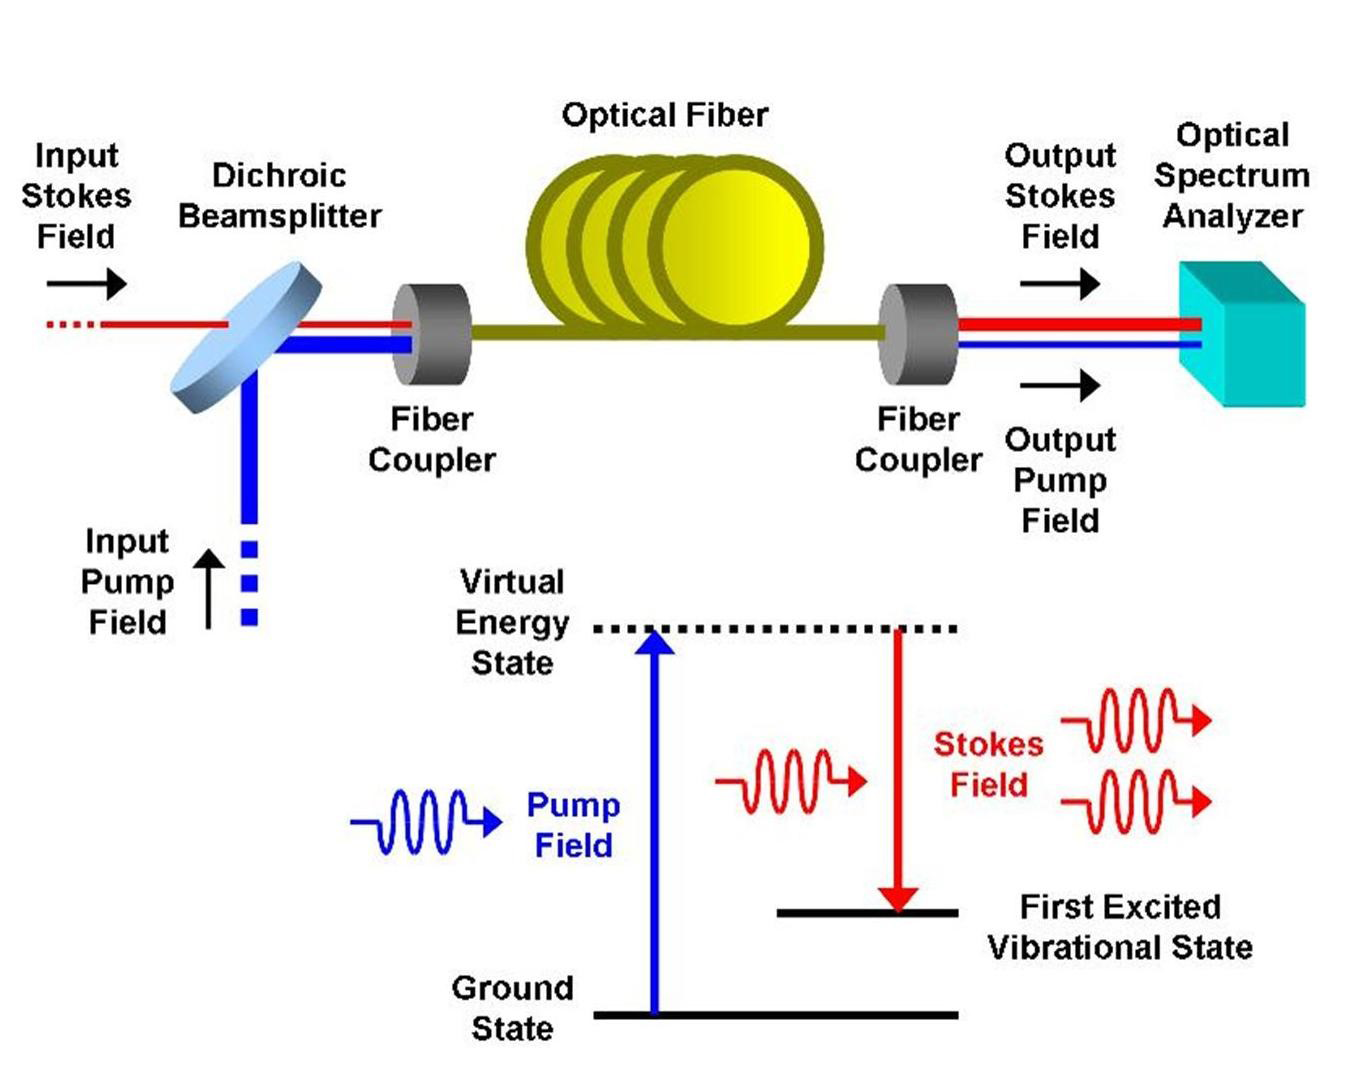
\includegraphics[scale=1]{APL_2011/Figure1.png}
\caption{Schematic of the STEAM vibrometer. The principle of the method is three-fold: (1) encoding of the lateral and axial coordinates of the target into the different frequencies and corresponding amplitudes of a spatially dispersed broadband pulse which spectrally interferes with a reference pulse, (2) amplified dispersive Fourier transformation in which the spectrum is mapped into a temporal waveform, time-stretched so that it can be digitized in real time, and simultaneously amplified in the optical domain, and (3) Hilbert transformation on the detected pulse in the digital domain to extract the axial information of the target.}
\label{fig:APL_2011_Figure1}
\end{figure}

The interferometrically combined pulses return to the same optics, but are directed via an optical circulator toward the amplified dispersive Fourier transformer (ADFT) [12, 13, 15] in which a dispersive fiber with -1200 ps/nm dispersion is optically pumped by four continuous-wave lasers with ~100 mW of optical power at 1470 nm, 1480 nm, 1480 nm, and 1490 nm for distributed Raman amplification. In the dispersive medium, the spectrum of each interfered pulse is stretched and converted into an amplified temporal waveform. This ADFT process is critical for high-speed laser vibrometry because the optical amplification before photon-to-electron conversion overcomes the fundamental trade-off between sensitivity and speed [12, 15]. The pulses are captured by a high-speed photodiode with 15 GHz bandwidth and digitized by a real-time oscilloscope with 16 GHz bandwidth and 50 GS/s sampling rate. Hilbert transformation is applied in the digital domain to each spectrally interfered pulse to obtain the axial information of the target at multiple points along the 1D line. Each pulse acquires one scan and the pulse repetition rate corresponds to the scan rate (frame rate) of the STEAM vibrometer.

The basic capabilities of the STEAM vibrometer (i.e., image pixel number, axial resolution, and dwell time) can be estimated from the parameters of its components. First, the number of image pixels on the target (N) is found from the total dispersion in the dispersive fiber (D = -1200 ps/nm), the optical bandwidth ( = 20 nm), and the sampling rate of the digitizer (fdig = 50 GS/s) to be N = |D|∙Δλ∙fdig = 1200 while the number of resolvable points is about 200 from the spectral resolution of the ADFT process [16]. Second, the axial resolution is given by the dynamic range (bit depth) of the digitizer. The axial resolution (z) can be found from the expression, 0.5sin(2kz) = 2-n, where k is the wavenumber [k = 2/(1590 nm)] and n is the bit depth of the digitizer (n = 8 bits), to be z = 0.99 nm. Finally, the dwell time is estimated from the bandwidth of each subpulse (20 nm / ~200) and the time-bandwidth product to be ~30 ps (assuming that the subpulses are transform limited).

We evaluated the basic performance of the STEAM vibrometer. In Figure 1-2a, the temporal waveform of a single interfered pulse captured by the photodiode is compared with the optical spectrum measured by a conventional optical spectrum analyzer. This verifies the equivalence of the two waveforms and hence validates the STEAM vibrometer. As shown in Figure 1-2b, repetitive pulses (scans) detected by the photodiode indicate that the STEAM vibrometer operates at 36.7 MHz scan rate.

\begin{figure}[htb!]
\centering
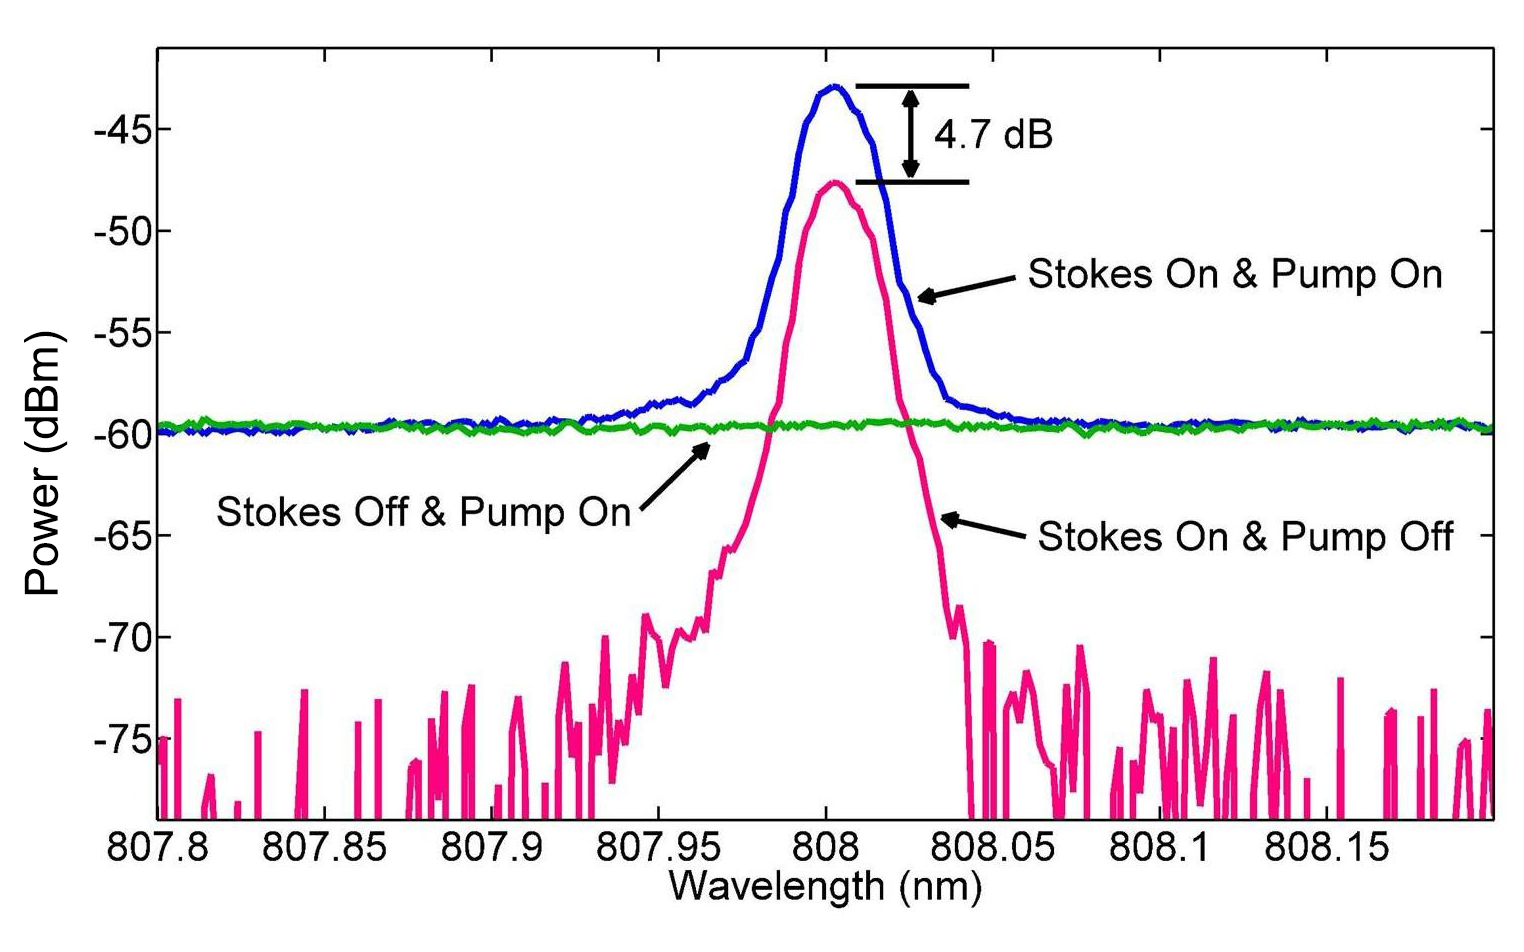
\includegraphics[scale=1]{APL_2011/Figure2.png}
\caption{Basic performance of the STEAM vibrometer. (a) Temporal waveform of a single interfered pulse captured by the photodiode in comparison with the optical spectrum measured by a conventional optical spectrum analyzer. (b) Repetitive pulses (scans) with a time interval of 27.2 ns detected by the photodiode indicating that the STEAM vibrometer operates at 36.7 MHz scan rate.}
\label{fig:APL_2011_Figure2}
\end{figure}

To show the utility of the STEAM vibrometer, we monitored the performance of an acoustic speaker. For better sensitivity, a thin reflective plate was attached to the diaphragm of the acoustic speaker. The speaker was driven up to 30 kHz (nearly its upper frequency limit). Figure 1-3 shows the 30 kHz surface vibration of the diaphragm captured by the STEAM vibrometer with ~1 nm axial resolution (which agrees with our estimated axial resolution of 0.99 nm).

\begin{figure}[htb!]
\centering
\includegraphics[scale=1]{APL_2011/Figure3.png}
\caption{Surface vibration of the acoustic diaphragm captured by the STEAM vibrometer with ~1 nm axial resolution and ~30 ps dwell time. The diaphragm was driven to vibrate at 30 kHz.}
\label{fig:APL_2011_Figure3}
\end{figure}

In addition to the amplitude of the surface vibration, we also obtained the velocity of the diaphragm from the axial coordinates of the surface as shown in Figure 1-4. The Doppler frequency shift in the frequency comb lines caused by the acoustic vibration (~830 Hz frequency shift) is negligible.

\begin{figure}[htb!]
\centering
\includegraphics[scale=1]{APL_2011/Figure4.png}
\caption{Axial velocity of the acoustic diaphragm obtained by the STEAM vibrometer. The diaphragm was driven to vibrate at 30 kHz (the same as in Figure \ref{fig:APL_2011_Figure3}).}
\label{fig:APL_2011_Figure4}
\end{figure}

In summary, we proposed and demonstrated an optical system that performs high-speed multi-dimensional imaging-based vibrometry and velocimetry with nanometer-scale axial resolution without the need for beam scanning. As a proof-of-concept, we showed real-time 1D imaging of fast acoustic vibrations with 1 nm axial resolution, 1200 image pixels, and 30 ps dwell time at 36.7 MHz scan rate. While we performed 1D cross-sectional imaging in this proof-of-principle demonstration, the technique can naturally be extended to 2D by using a 2D spatial disperser [12, 16].

                         % Chapter 2
%\input {chapter3}                         % etc.
%\input {chapter4}
%\input {Conclusion}

%\bibliography {bib/network,bib/naming}    % bibliography references
%\bibliographystyle {thesis}

%\bibliographystyle {IEEEtran}
%\bibliography {IEEEfull,DissertationBib} 

\bibliography{DissertationBib}
\bibliographystyle{unsrt}

\end {document}
